\documentclass[12pt, a4paper]{article}

\usepackage{graphicx}
\usepackage{capt-of}
\usepackage{hyperref}

\setlength{\oddsidemargin}{0.5cm}
\setlength{\evensidemargin}{0.5cm}
\setlength{\topmargin}{-1.6cm}
\setlength{\leftmargin}{0.5cm}
\setlength{\rightmargin}{0.5cm}
\setlength{\textheight}{24.00cm} 
\setlength{\textwidth}{15.00cm}

\def\myname{Richard Ogujawa}
\parindent 0pt
\parskip 5pt

\pagestyle{plain}

    \title{\textbf{Research Proposal}}
\author{Richard Ogujawa (L00145067)}
\date{\today}


\newcommand{\namelistlabel}[1]{\mbox{#1}\hfil}
\newenvironment{namelist}[1]{%1
\begin{list}{}
    {
        \let\makelabel\namelistlabel
        \settowidth{\labelwidth}{#1}
        \setlength{\leftmargin}{1.1\labelwidth}
    }
  }{%1
\end{list}}

\begin{document}
\maketitle

\begin{namelist}{xxxxxxxxxxxx}
\item[{\bf Title:}]
	Using Machine Learning to Help Reduce Road Accidents
\item[{\bf Supervisor:}]
	Professor Shagufta Henna 
\item[{\bf Degree:}]
	MSc Data Science
\end{namelist}

\section*{Problem Description}Machine learning (ML) has been utilized in many different ways over the years to solve a variety of problems: From helping businesses figure out how to increase revenue by dynamically adjusting their prices based on market trend analysis, to placing medical professionals in a better position to save lies through faster and more accurate diagnoses. However, an ML model is only as good as the data provided it. As such unreliable data, or a lack of data in general, naturally impedes upon the prospect of being able to properly implement ML solutions. \\
Such was the case in New York City with regards to the lack of access to open traffic crash data, until a breakthrough occurred:
\begin{quote}
    "After years of prodding from safe streets advocates, the New York City Council, and the tech community — not to mention reporters — New York City has finally released comprehensive traffic crash data." (WNYC, 2014)
\end{quote}

This is important because according to a report by the Centers for Disease Control and Prevention (CDC), it's estimated that over 1.35 million people lose their lives on the road globally, with a daily estimate of 3,700 deaths worldwide. Speaking to the situation in the US specifically, the report claims that road accidents are the eighth leading cause of death and the number one leading cause of unnatural death. (CDC, 2019)

However, with access to data like the one that WYNC is referring to (which is the one that will be used  in this research project), solutions can be created to help tackle the issue and bring the number of deaths to a minimum. For example, smart cars could analyse the time of day, take note of the car's location, and utilise other factors to help predict the likelihood of a car crash and tell the driver of the vehicle to drive more cautiously if its predictions warrant such.

Some other ideas which have already been explored regarding the reduction of road accidents include: 
\begin{itemize}
    \item \textbf{Head-Up Displays:} In a university paper by Muhammad Saffarini, Rasha Saffarini and Isam Ishaq, an idea was proposed to help fight against one of the causes of road accidents - drowsiness. They created a system to help achieve this using technology like Raspberry Pi, Arduino, C++, Python, PHP and SQL. How the system works is that it: 
    \begin{quote}    
        "...continuously detects the driver's head motion, yawning, and blinking from instantaneous video. The detected motions are passed to a classifier which predicts if the driver is asleep or not. The accuracy of prediction reached around" 90\%. (Saffarini, Saffarini, Ishaq, 2020)
    \end{quote} 
    \begin{center}
        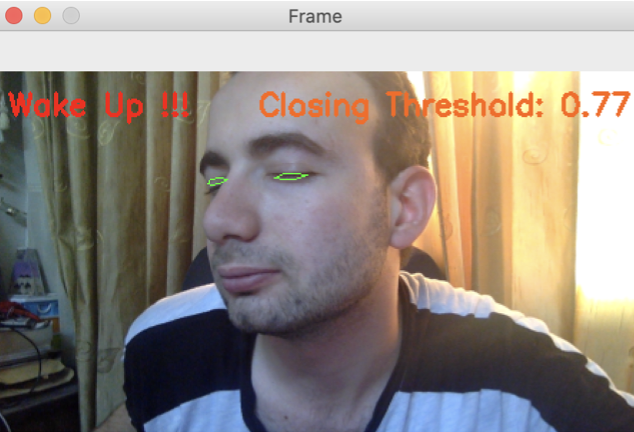
\includegraphics[width=0.5\linewidth]{The side view of the face and eyes are closed.png}
        \captionof{figure}{Program detecting eyes closed on side view of a face.}
        \label{fig:side-view-eyes-closed}
    \end{center}
    
    \item\textbf{Smart Car Systems:} Self-driving is also currently being explored as a solution to reduce road accidents. One of the breakthroughs so far is the creation of car systems which are designed to ensure that the car is aware of its surroundings: Laser sensors are used to do 360-degree scans of its environment to detect vehicles and other objects, radars are used to measure the speed of vehicles ahead, etc. These system, with all the information they gather, are then able to make better decisions with regard to navigating the vehicle on behalf of the driver. (Sagar and Choudhary, 2020)
\end{itemize}

\section*{Goals} As death is arguably the most tragic consequence of a road accident, this research project will be anchored around that. During the course of this project, questions will be asked of the dataset in order to better understand the factors which contribute most to death being an outcome. The questions this predictive model seeks to answer include the following - Can we predict whether or not a death is likely to occur given: (1) The day of the week? (2) The time of the day? (3) The location? (3) The month? (4) Any combination of day, time and location? (4) the type of vehicles involved in the incident? (5) The number of vehicles involved in the incident?, etc. 

The predictions will be Boolean in nature, i.e. True or False.


\section*{Dataset Description}
The dataset which will be used in this project is the \href{https://data.cityofnewyork.us/Public-Safety/Motor-Vehicle-Collisions-Crashes/h9gi-nx95}{'Motor Vehicle Collisions - Crashes' table}, which contains information about crashes that occurred in New York City (NYC). Sourced from NYC police reports, the dataset comprises 2.03 million rows and 29 columns. Each record is a singular road crash incident and each column/attribute provides more and more details about the crash. The attributes present include descriptors like the time and date of the crash, where the crash happened, and finally the nature of the incident with regards to how many vehicles/people were involved. Also, each crash is uniquely identified by the collision\_id attribute. 

Given the aforementioned goals for this project, the column which is most apt to act as the label/golden standard will be a generated column called "Did Someone Die" which will be created based on the "Number of Persons Killed" field which, as the name suggests, stores discrete numeric data specifying the number of human deaths that occurred as a result of the accident being detailed on that particular row. If the value under the "Number of Persons Killed" column is greater than 0, then the "Did Someone Die" column, for that particular row, will get a value of 1. The generated column is necessary because there is no column with categorical data which plainly specifies whether or not a death occurred which is paramount for the model to be able to answer the questions posed in the Goal's section of this paper. Also, the following columns have been selected as features to help answer the questions posed in the Goals section of this paper: crash date, crash time, borough, zip code, on street name, contributing factor vehicle 1, contributing factor vehicle 2, contributing factor vehicle 4, contributing factor vehicle 5, vehicle type code 1, vehicle type code 2, vehicle type code 3, vehicle type code 4, vehicle type code 5.

The only real challenge the dataset seemed to pose initially was the presence of missing values, however upon further inspection, it's evident that unless all the features in a row contain missing values, the observation is still useful.

\section*{Methodology}
The implementation of an Analytic Pipeline will most likely resemble the structure demonstrated in the figure below - Figure 2: 
\begin{center}
    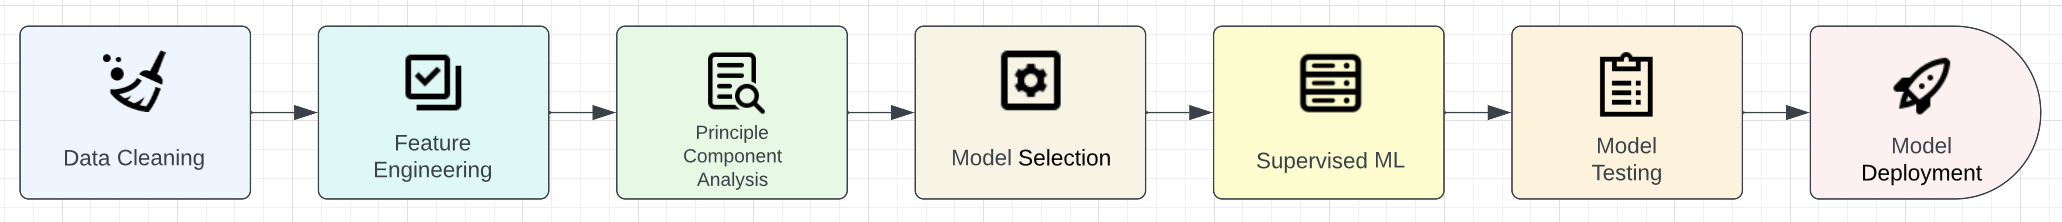
\includegraphics[width=\linewidth]{Analytic Pipeline.png}
    \captionof{figure}{Proposed Analytic Pipeline}
    \label{fig:analytic-pipeline}
\end{center}
The data will be imported from the dataset and then cleaned up and wrangled in the Data Transformation stage in order to prepare it for use in the model to produce desirable predictions. However, before it can be used to train ML algorithms into a model, the dataset needs to be whittled down to only include the columns necessary to make useful/accurate predictions - i.e. feature engineering. Then Principle Component Analysis will be applied to improve the quality of the features. Finally the data can be passed into the Supervised ML Algorithms stage where it will be used to train the chosen classifier into a useful model suitable for making appropriate predictions. This enabled the undergoing of predictive analysis which will be where the questions in the Goals section of this paper will be answered. 

In terms of the predictive model being chosen to be trained in the Supervised ML stage, the following options were chosen \href{https://scikit-learn.org/stable/modules/ensemble.html#random-forests-and-other-randomized-tree-ensembles}{Random Forests} and \href{https://scikit-learn.org/stable/modules/ensemble.html#bagging-meta-estimator}{Bagging Meta-Estimator}:
The choice came down to the following: 
\begin{itemize}
    \item The questions that the predictive model seek to answer are all classification problems, as such it was imperative that the chosen choice of predictive models each had to come with a classifier class, and both of the aforementioned algorithms do.
    \item Also, the fact that the predictive model is going to be used to hopefully alter behaviour to help prevent road deaths, a sense of stability in the estimations was of utmost importance. As such, a low degree of variance was highly desirable, which is a key feature in both of the algorithms. According to the documentation Random Forests reduces variance by combining diverse trees; the Bagging Estimator algorithm, achieves the same outcome via the introduction of  randomization into its construction procedure, of which it then makes an ensemble. (Sci-kit learn, 2023)
\end{itemize}

\section*{References}
\begin{enumerate}
\item WNYC. (2014). NYC Open Traffic Crash Data -- Finally | WNYC | New York Public Radio, Podcasts, Live Streaming Radio, News. [online] Available at: \href{https://www.wnyc.org/story/nyc-opens-traffic-crash-data-finally/}{https://www.wnyc.org/story/nyc-opens-traffic-crash-data-finally/} [Accessed 19 Oct. 2023].
\item CDC (2019). Global Road Safety. [online] Centers for Disease Control and Prevention. Available at: \href{https://www.cdc.gov/injury/features/global-road-safety/index.html\#:~:text=Each%20year%2C%201.35%20million%20people} [Accessed 19 Oct. 2023]{https://www.cdc.gov/injury/features/global-road-safety/index.html\#:~:text=Each\%20year\%2C\%201.35\%20million\%20people.}.
‌\item Muhammed Saffarini, Rasha Saffarini and Isam Ishaq. (2020). Smart System to Avoid Car Accidents. doi:\href{https://doi.org/10.1109/ICPET51420.2020.00013}{https://doi.org/10.1109/ICPET51420.2020.00013}
‌\item Anil Kumar Sagar, Ankur Choudhary (2020). Smart Car System: Review [online] Available at: \\ \href{https://www.jcreview.com/admin/Uploads/Files/61a593019260b5.18878346.pdf}{https://www.jcreview.com/admin/Uploads/Files/61a593019260b5.18878346.pdf} [Accessed 19 Oct. 2023].
\item Sci-kit learn (2023). 1.11. Ensembles: Gradient boosting, random forests, bagging, voting, stacking [online] Available at: \href{https://scikit-learn.org/stable/modules/ensemble.html\#bagging-meta-estimator}{https://scikit-learn.org/stable/modules\\/ensemble.html\#bagging-meta-estimator} [Accessed 27 Oct. 2023].
‌

‌\end{enumerate}

\end{document}

